\documentclass[../../main.tex]{subfiles}

\graphicspath{{../../fig/}}
\setcounter{section}{0}

\begin{document}
\chapter{スパースワイヤーグリッドのたわみ量の評価}
\label{chap:wiresag_swg}
\ref{chap:wiresag}章にて、ワイヤーのたわみ量を自動で評価する装置を開発した。
本章では、開発した装置を用いて実際に偏光角較正に使用されるスパースワイヤーグリッドのたわみ量を評価する。
はじめに、評価するスパースワイヤーグリッドのワイヤーの張り方について述べ、次いで評価結果とその考察を行う。
その後、評価されたたわみ量が大きかったものについて修繕を加え、再度評価を行った結果について述べる。
最後に、今回のたわみ量の評価を通じて得られた、スパースワイヤーグリッドの作成方法に関する今後の展望について述べる。

\section{評価されたスパースワイヤーグリッドのワイヤーの張り方}
今回評価したスパースワイヤーグリッドは、\ref{subsec:wg_design}項で述べたように$\SI{230}{g}$の重りを使用し、
ワイヤー番号が奇数番目のものと偶数番目のものに分け、二回に分けてワイヤーを張ることで作成された。
このとき、はじめにワイヤー番号が奇数番目のものを張り、次にワイヤー番号が偶数番目のものを張った。
作成されたスパースワイヤーグリッドを装置に取り付けた様子を図\ref{fig:wiresag_swg_sparse_wiregrid}に示す。
なお、\ref{chap:wiresag}章にて述べたように一度に測定できるのはスパースワイヤーグリッドの半面のみであるので、
ワイヤー番号が$0\sim19$番のワイヤーと$20\sim38$番のワイヤーに分けて測定を行った。

\section{評価結果とその考察}
図\ref{fig:wiresag_swg_result}(\subref{fig:wiresag_swg_sag_result})にスパースワイヤーグリッドのたわみ量の評価結果を示す。
横軸はワイヤー番号、縦軸はワイヤーのたわみ量を示している。
fitting errorを統計的な誤差として、前章にて得られた$\SI{50}{\micro m}$を系統的な誤差として、それらの2乗和の平方根をたわみ量の誤差として示した。
図中には測定されたたわみ量に加え、理論値として$\SI{230}{g}$の重りによって生まれるたわみ量(平均たわみ角にして$0.006\tcdegree$)を、
たわみ角が$0.3\tcdegree,\,0.5\tcdegree$になるたわみ量を示している。
図\ref{fig:wiresag_swg_result}(\subref{fig:wiresag_swg_sag_angle_result})に
評価されたたわみ量をたわみ角に変換した結果を示す。
横軸はワイヤー番号、縦軸はワイヤーのたわみ角を示している。
図中には測定されたたわみ角に加え、たわみ角が$0.03\tcdegree,\,0.05\tcdegree$の線を示している。
測定されたたわみ角の平均は$0.025\tcdegree$である。

また、明らかにたわみ量が大きく、たわみ角が$0.05\tcdegree$を超えるワイヤーが存在していた。
これらのワイヤーはすべて奇数番目のワイヤーであった。
図\ref{fig:wiresag_swg_even_odd}にワイヤー番号の偶奇によるたわみ量の違いを示す。
偶数番目のワイヤーのたわみ量を青点で示し、奇数番目のワイヤーのたわみ量を赤点で示している。
この図より、奇数番目のワイヤーのたわみ量が偶数番目のワイヤーに比べて大きい傾向にあることがわかる。
今回評価したスパースワイヤーグリッドは奇数番目のワイヤーから張り始めたことから、このたわみ量の違いは、
\begin{enumerate}
    \item 単に奇数番目のワイヤーを張るときにうまく張れなかった
    \item 後に張ったワイヤーによる張力によってスパースワイヤーグリッドのアルミニウムリングが歪み、
          先に張ったワイヤーがたわんでしまった
\end{enumerate}
の2つの可能性が考えられる。
そこで、奇数番目のワイヤーのみを張り直し、修繕することによりたわみ量がどう変化するかを調べることで、
上記2つの可能性のうちどちらが実際に起きているのかを明らかにする。
\begin{figure}[H]
    \begin{minipage}[b]{0.5\hsize}
        \centering
        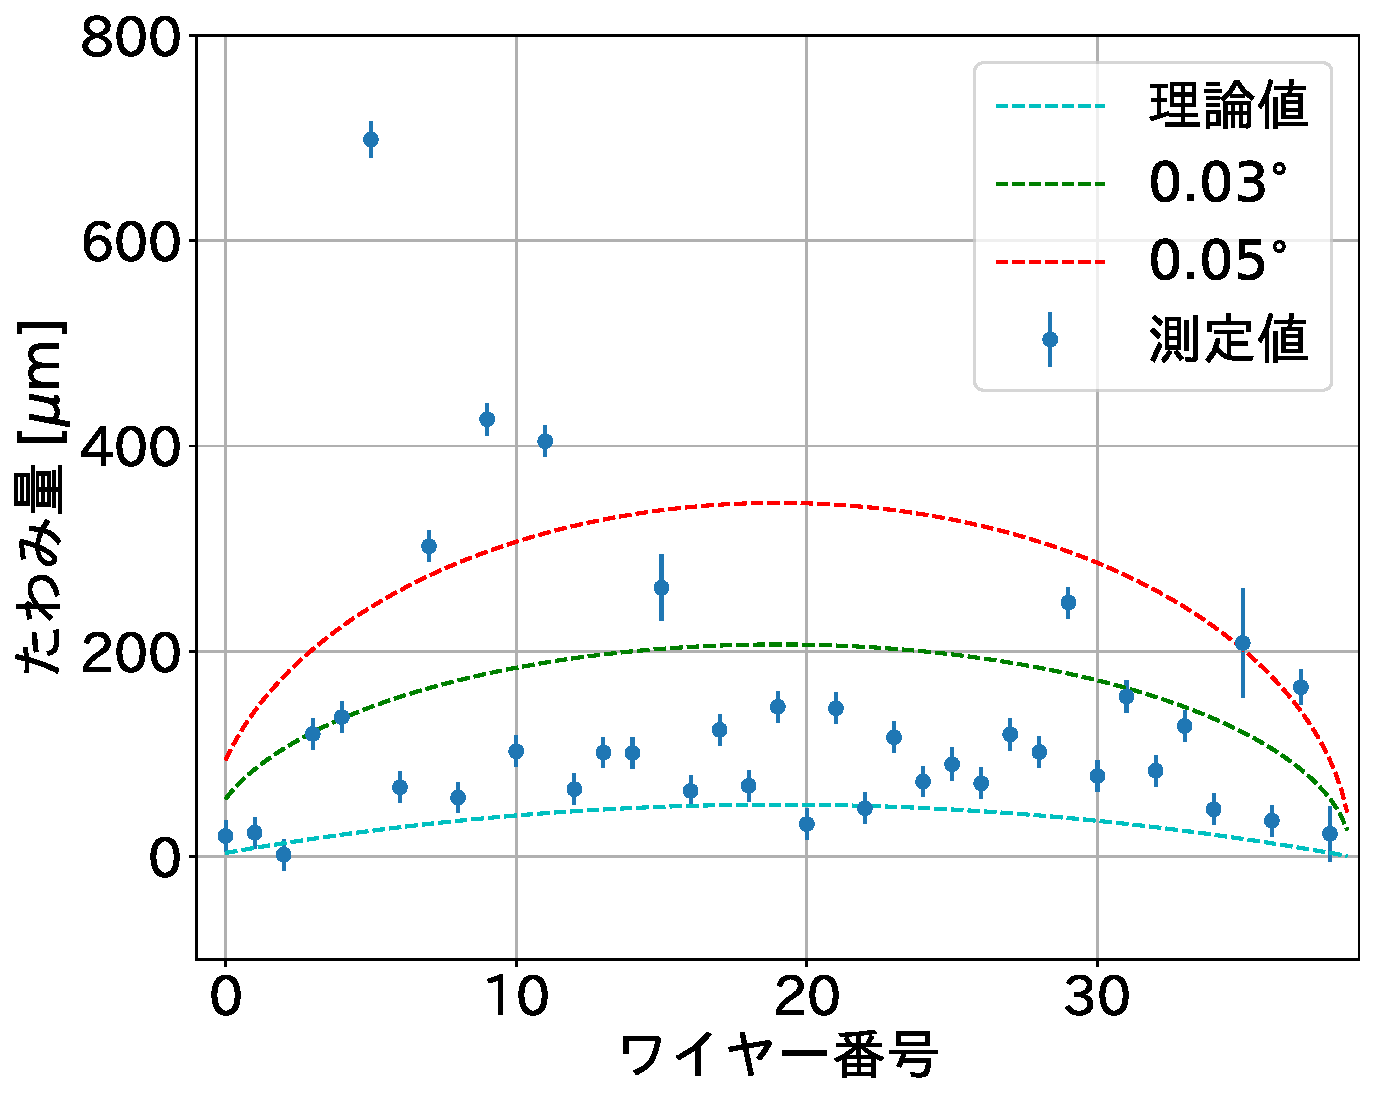
\includegraphics[width=1.0\textwidth]{wiresag_swg/swg_sag_before.pdf}
        \subcaption{}
        \label{fig:wiresag_swg_sag_result}
    \end{minipage}
    \begin{minipage}[b]{0.5\hsize}
        \centering
        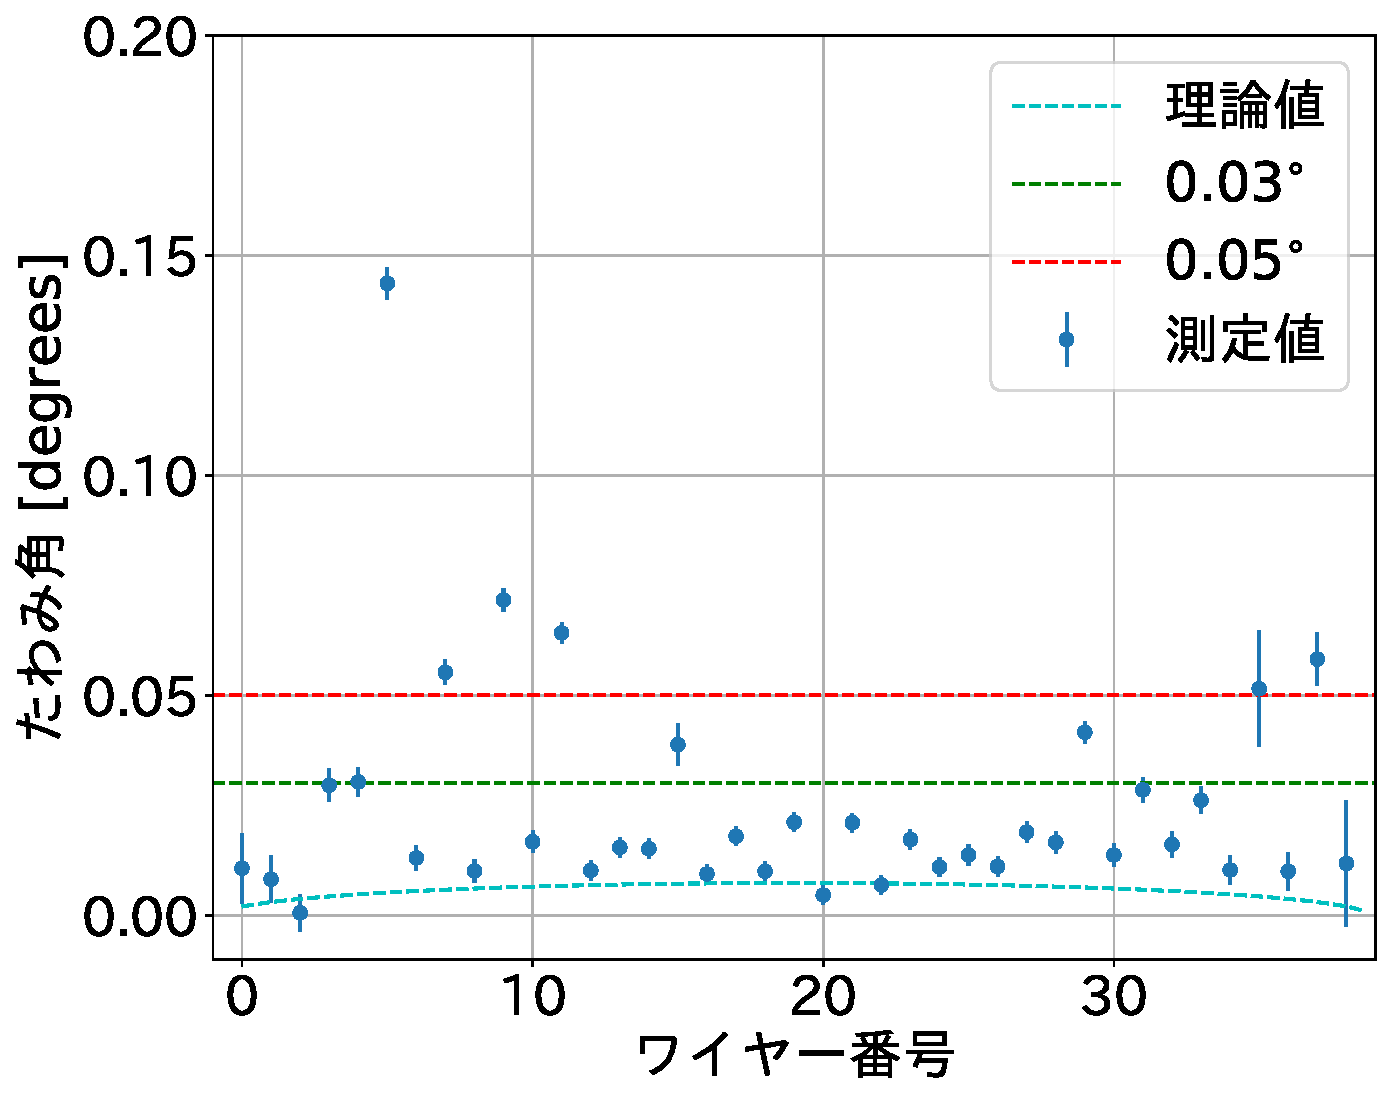
\includegraphics[width=1.0\textwidth]{wiresag_swg/swg_sag_angle_before.pdf}
        \subcaption{}
        \label{fig:wiresag_swg_sag_angle_result}
    \end{minipage}
    \caption{(\subref{fig:wiresag_swg_sag_result}) スパースワイヤーグリッドのたわみ量の評価結果。\ 
             (\subref{fig:wiresag_swg_sag_angle_result}) たわみ量を角度に変換したもの。}
    \label{fig:wiresag_swg_result}
\end{figure}
\begin{figure}[H]
    \centering
    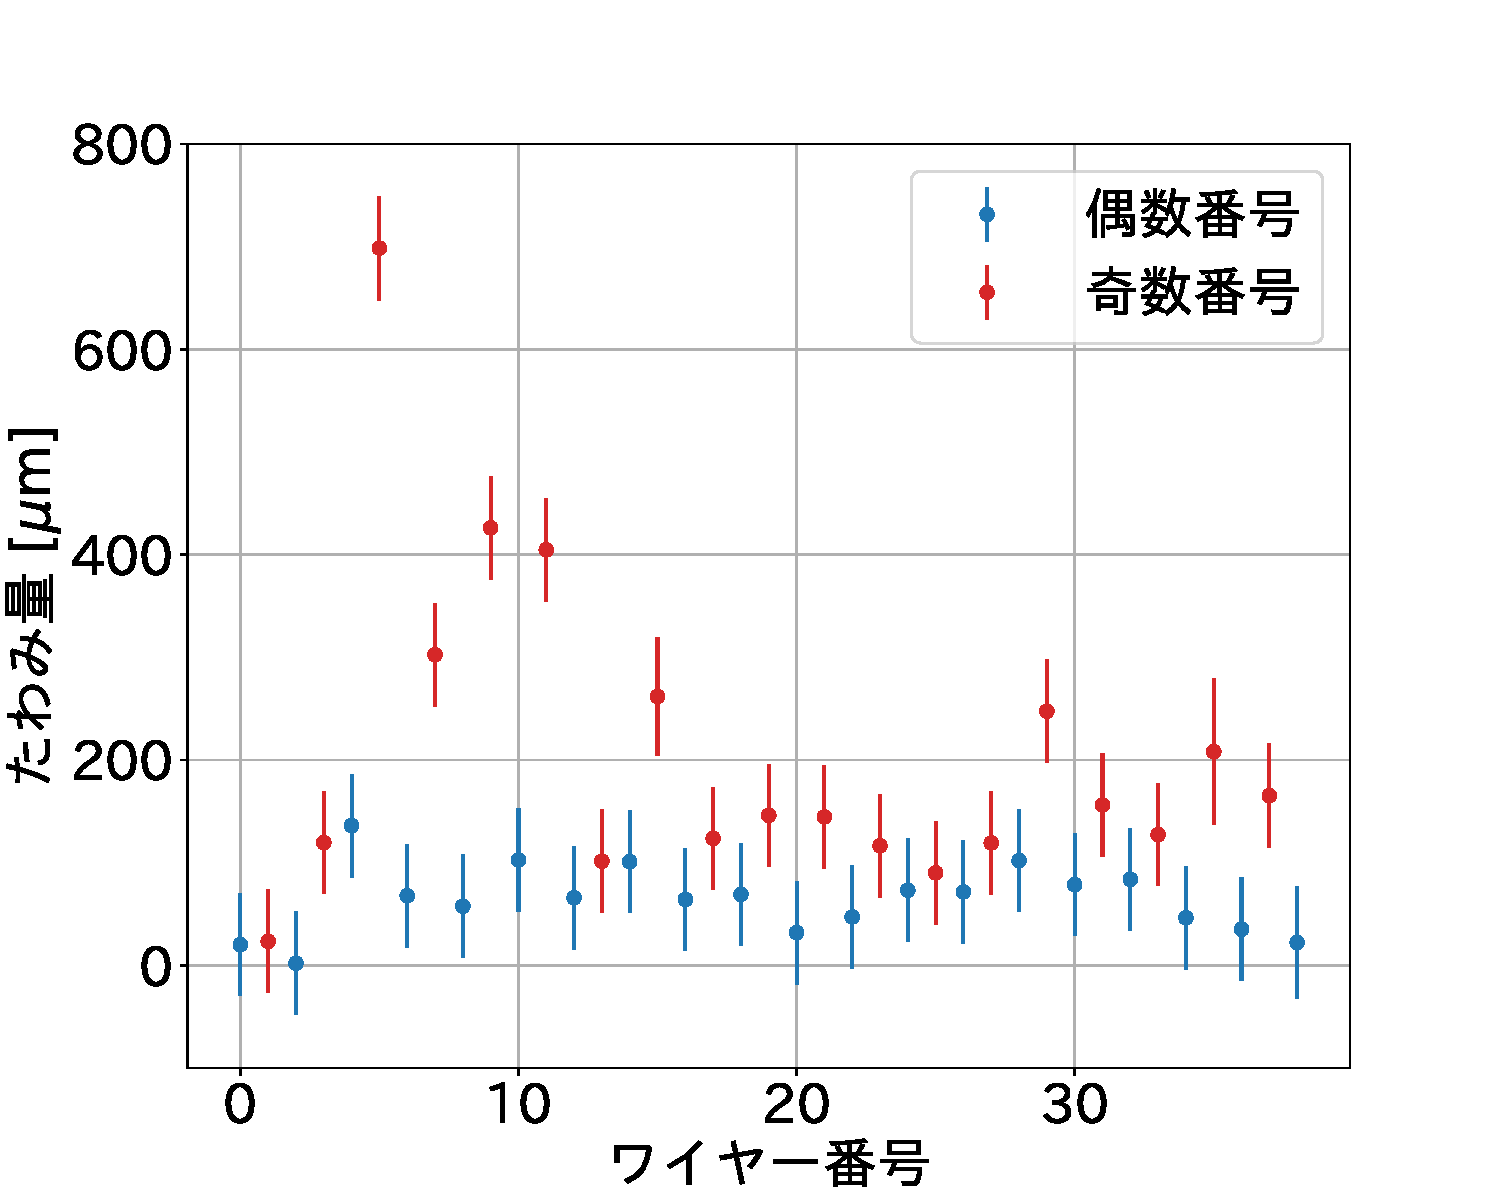
\includegraphics[width=0.8\textwidth]{wiresag_swg/swg_sag_before_even_odd.pdf}
    \caption{ワイヤー番号の偶奇によるたわみ量の違い。全体的に奇数番号のワイヤーの方が偶数番号のワイヤーと比較してたわみ量が大きい傾向にある。}
    \label{fig:wiresag_swg_even_odd}    
\end{figure}

\section{修繕後のスパースワイヤーグリッドの評価}
奇数番目のワイヤーを切り、再度張り直すことで修繕されたスパースワイヤーグリッドのたわみ量を評価した。
修繕後のスパースワイヤーグリッドのたわみ量の評価結果を図\ref{fig:wiresag_swg_result_repair}(\subref{fig:wiresag_swg_sag_result_repair})に、
たわみ角の評価結果を図\ref{fig:wiresag_swg_result_repair}(\subref{fig:wiresag_swg_sag_angle_result_repair})に示す。
どちらの図中にも、比較のために修繕前の評価結果もあわせて示している。
得られたたわみ角の平均は$0.020\tcdegree$であり、修繕前のたわみ角の平均$0.025\tcdegree$よりも$0.005\tcdegree$改善した。
また、修繕前にたわみ角が$0.05\tcdegree$を超えるワイヤーは6本存在していたが、修繕後には2本に減少している。
この結果は、本装置を用いてワイヤーのたわみ量を評価することにより、品質の悪いワイヤーを張り直してたわみ量を改善可能であることを示している。

% 修繕前後での評価されたワイヤーのたわみ量の比較を図\ref{fig:wiresag_swg_result_repair_compare}に示す。
% また、たわみ角についても同様に比較した図を図\ref{fig:wiresag_swg_result_repair_angle_compare}に示す。

% したがって、これらの和をとることにより修繕後のワイヤーのたわみが与える望遠鏡の偏光角較正への影響は
% $\theta_{\mathrm{sag}}=0.030\tcdegree$であり、修繕前の$\theta_{\mathrm{sag}}=0.036\tcdegree$よりも小さくなった。

また、図\ref{fig:wiresag_swg_even_odd_repair}に修繕後のワイヤーについて、ワイヤー番号の偶奇によるたわみ量の違いを示す。
青点が偶数番目のワイヤーのたわみ量を示し、赤点が奇数番目のワイヤーのたわみ量を示している。
修繕後のワイヤーに関しては、奇数番目よりも偶数番目のワイヤーのたわみ量が大きくなっており、
修繕前の傾向と逆の傾向を示した。
図\ref{fig:wiresag_swg_even_odd_repair_comparison}(\subref{fig:wiresag_swg_sag_odd_comparison})に奇数番目のワイヤーのたわみ量を修繕前後で比較した結果を、
図\ref{fig:wiresag_swg_even_odd_repair_comparison}(\subref{fig:wiresag_swg_sag_even_comparison})に偶数番目のワイヤーのたわみ量を修繕前後で比較した結果を示す。
これらの図から、ワイヤーのたわみ量を修繕前後では奇数番目は修繕によりたわみ量が小さくなっているが、偶数番目は修繕後の方が大きくなっていることがわかる。
修繕は奇数番目のワイヤーのみを張り直すことで行われたため、スパースワイヤーグリッドのワイヤーは2回に分けて張ることにより、先に張られたワイヤーがたわんでしまうことがわかった。

2本品質の悪いワイヤーはあるものの、今回の修繕後の結果を用いて、ワイヤーのたわみに起因する望遠鏡の偏光角較正への影響を算出する。
修繕後のワイヤーのたわみ角の平均値は$0.020\tcdegree$(これは品質の悪い2本を入れた値であり、それらを除くと$0.015\tcdegree$)、たわみ角の誤差の平均値は$0.010\tcdegree$であった。
先行研究にしたがい、これらの和をありうる最大のたわみ角とすると、$\theta_{\mathrm{sag}}<0.030\tcdegree$といえる。
よって、先行研究で得られた$\theta_{\mathrm{sag}}<0.05\tcdegree$よりも$40\%$たわみによる偏光角較正の誤差を改善することができた。
% 明らかに品質の悪い$4,\,6$番目の以外の偶数番目のワイヤーで、修繕前後のたわみ角の変化の平均値を算出すると$0.01\tcdegree$であった。



\begin{figure}[H]
    \begin{minipage}[b]{0.5\hsize}
        \centering
        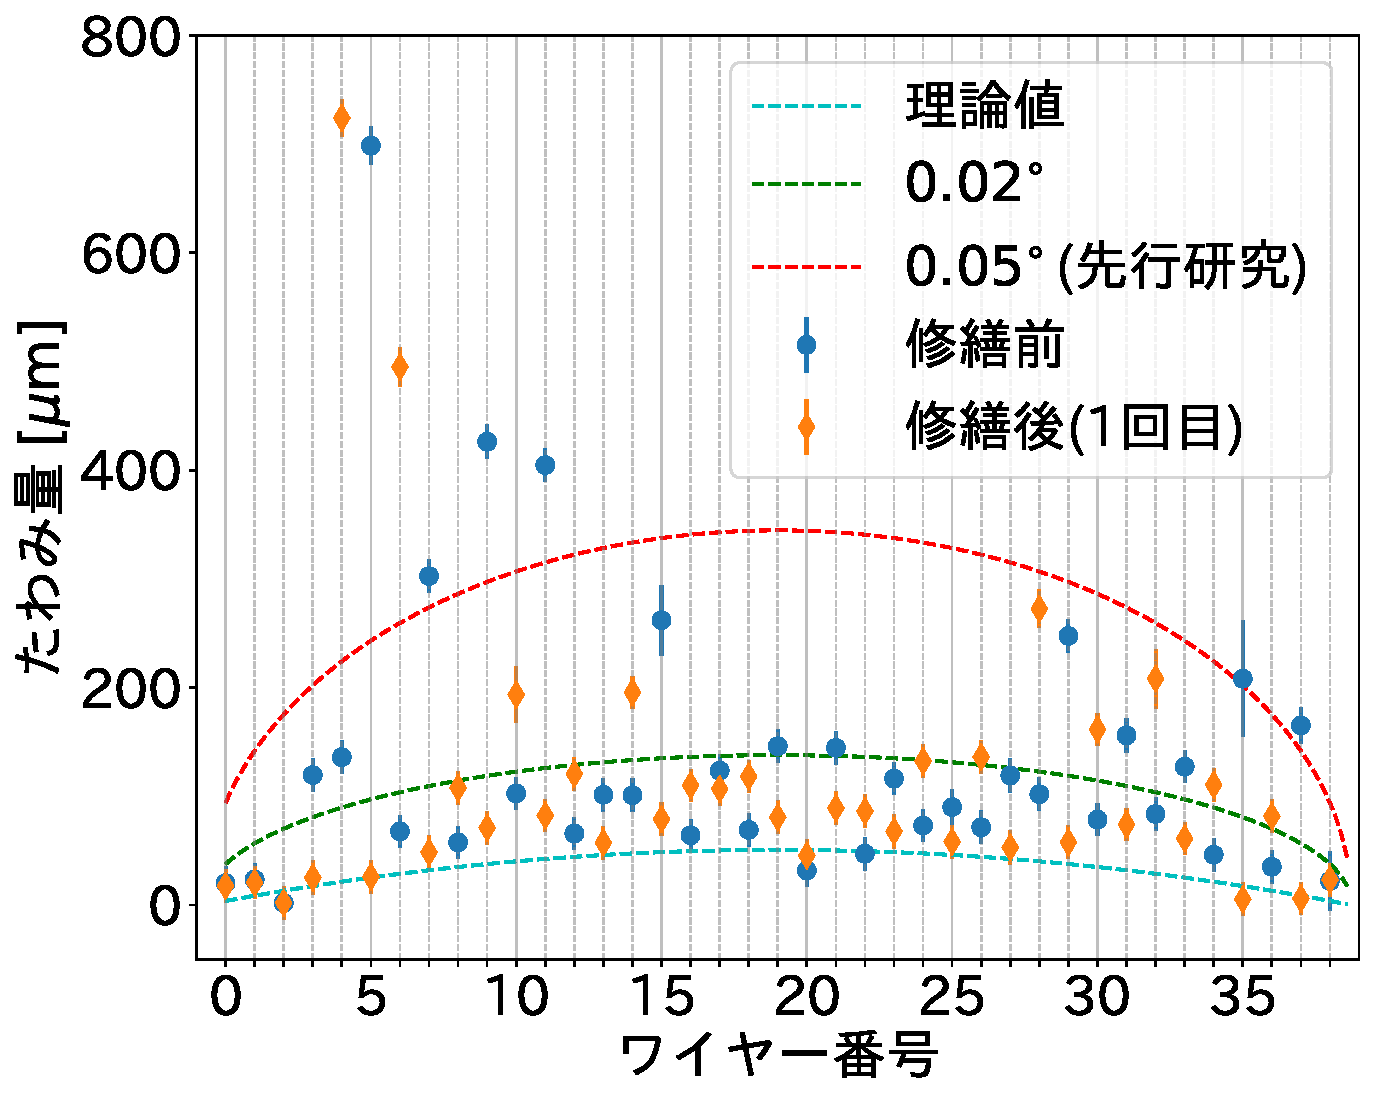
\includegraphics[width=1.0\textwidth]{wiresag_swg/swg_sag_comparison.pdf}
        \subcaption{}
        \label{fig:wiresag_swg_sag_result_repair}
    \end{minipage}
    \begin{minipage}[b]{0.5\hsize}
        \centering
        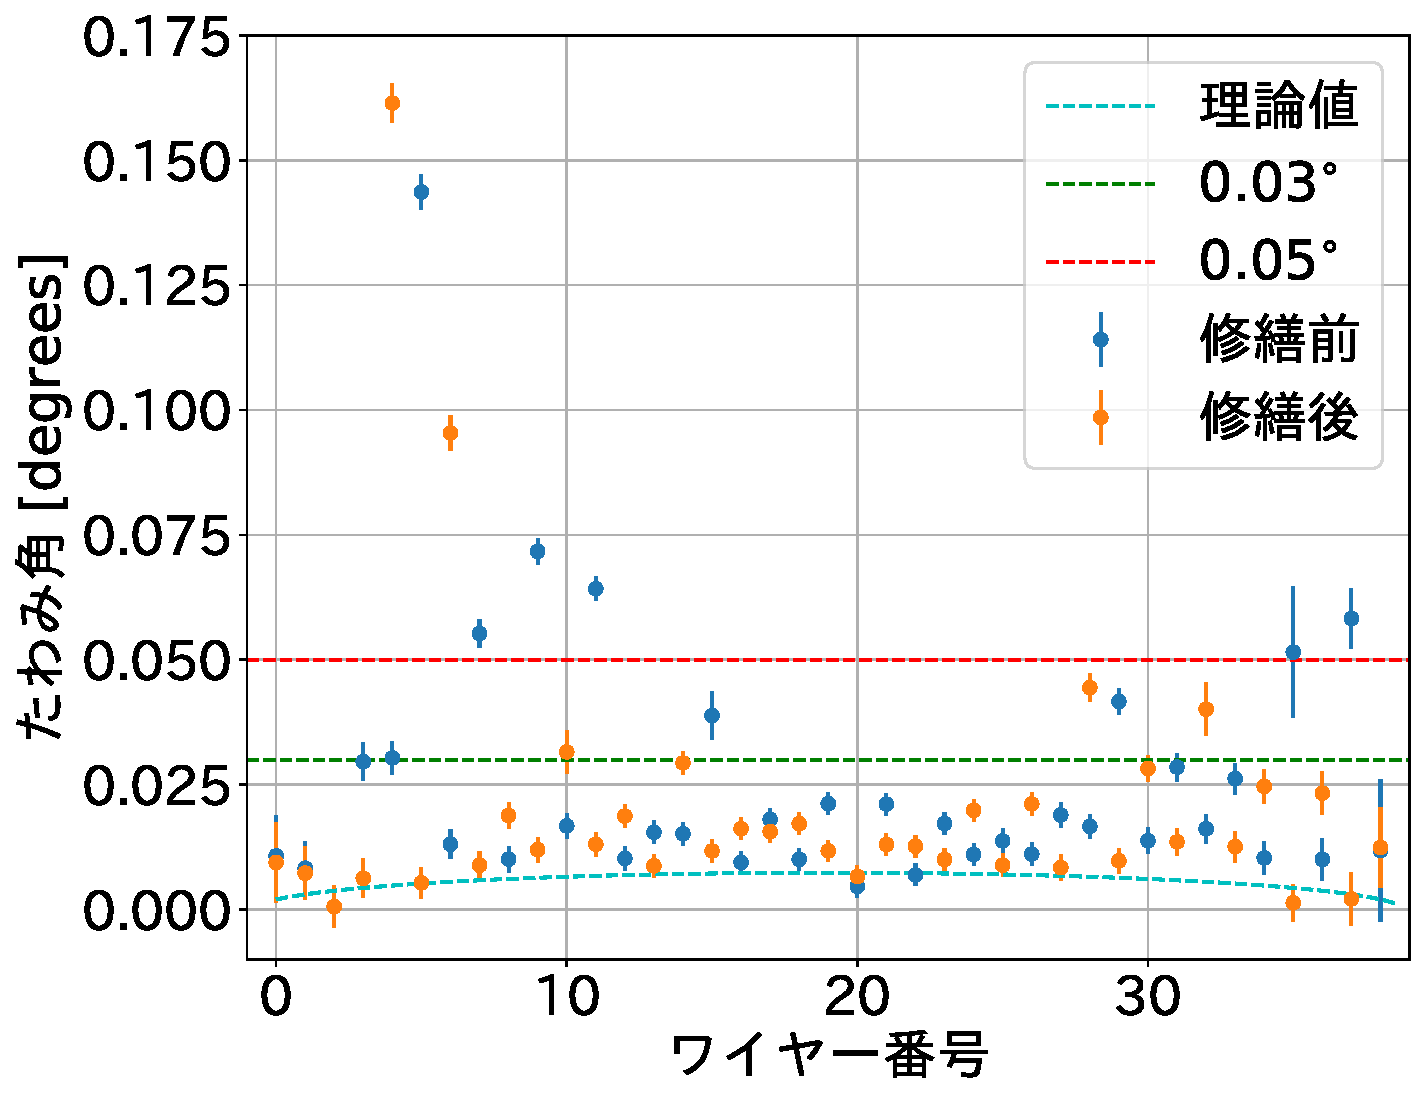
\includegraphics[width=1.0\textwidth]{wiresag_swg/swg_sag_angle_comparison.pdf}
        \subcaption{}
        \label{fig:wiresag_swg_sag_angle_result_repair}
    \end{minipage}
    \caption{(\subref{fig:wiresag_swg_sag_result_repair}) 修繕後のスパースワイヤーグリッドのたわみ量の評価結果。\ 
             (\subref{fig:wiresag_swg_sag_angle_result_repair}) 修繕後のスパースワイヤーグリッドのたわみ角の評価結果。
             $0.05\tcdegree$を超えるたわみ角を有していたワイヤーが修繕により改善されている。}
    \label{fig:wiresag_swg_result_repair}
\end{figure}
\begin{figure}[H]
    \centering
    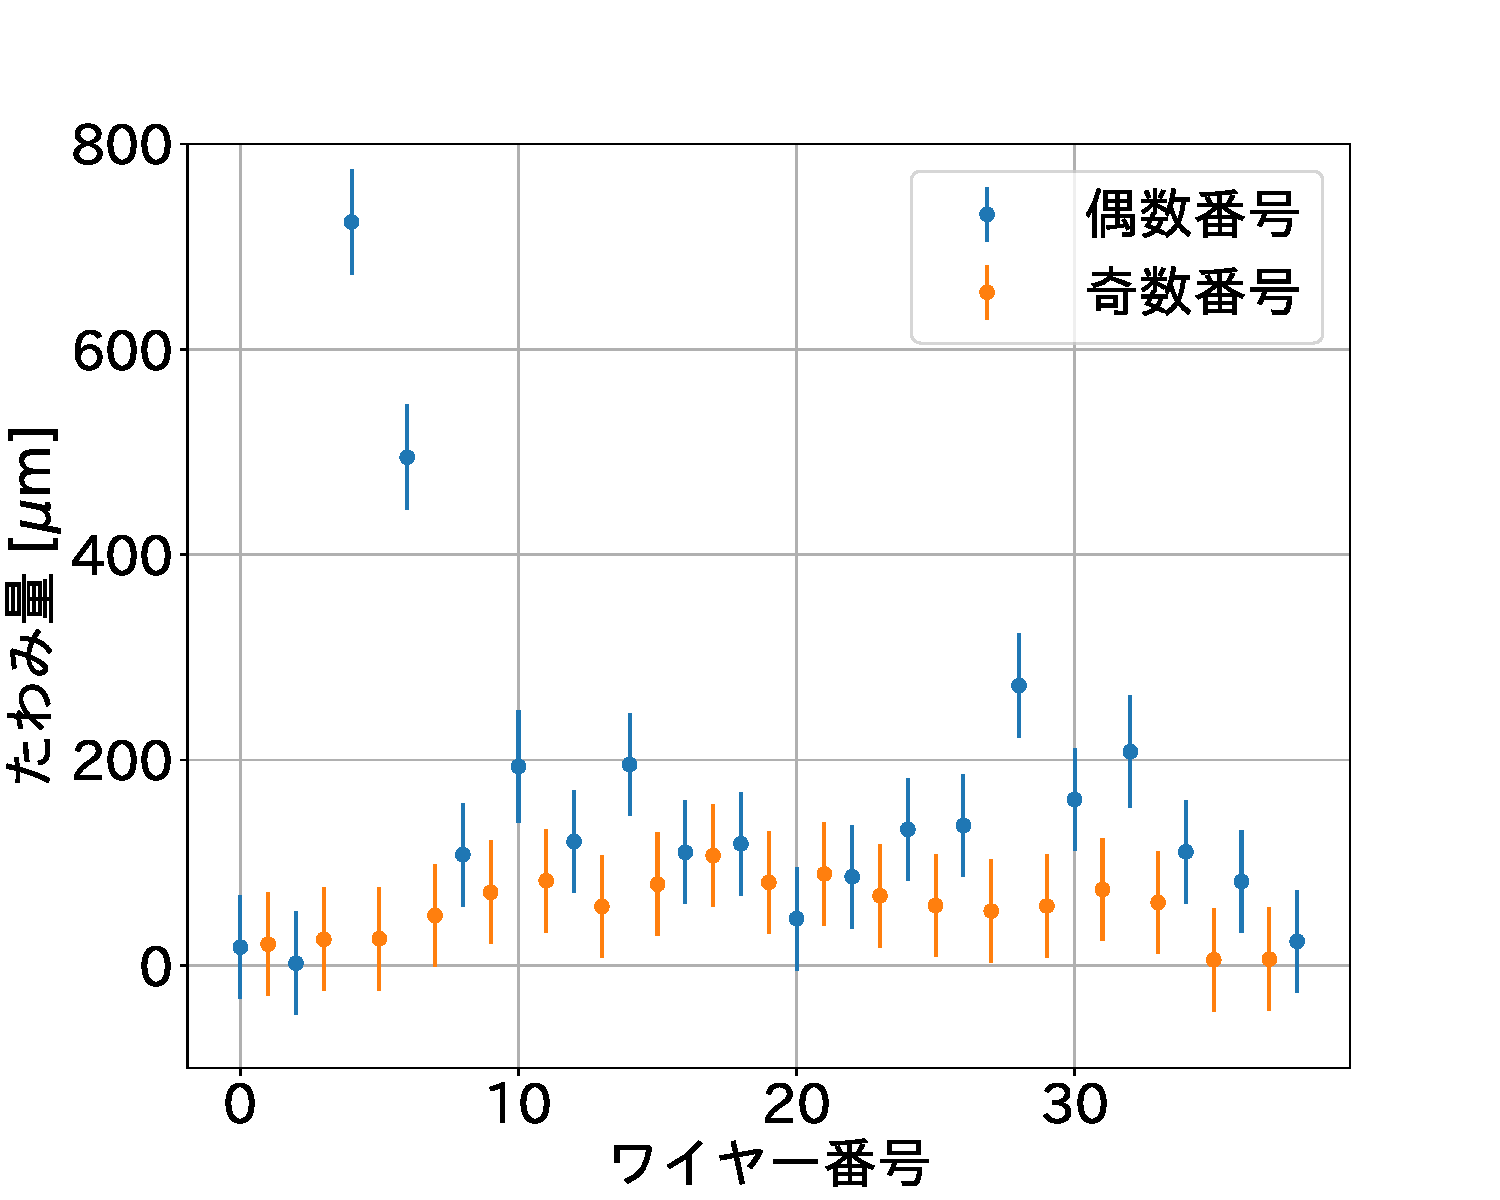
\includegraphics[width=0.8\textwidth]{wiresag_swg/swg_sag_after_even_odd.pdf}
    \caption{修繕後のワイヤー番号の偶奇によるたわみ量の違い。
    偶数番号のワイヤーの方が奇数番号よりも大きなたわみ量を示している。
    これは修繕前の図\ref{fig:wiresag_swg_even_odd}と逆の傾向を示している。}
    \label{fig:wiresag_swg_even_odd_repair}
\end{figure}
\begin{figure}[H]
    \begin{minipage}[b]{0.5\hsize}
        \centering
        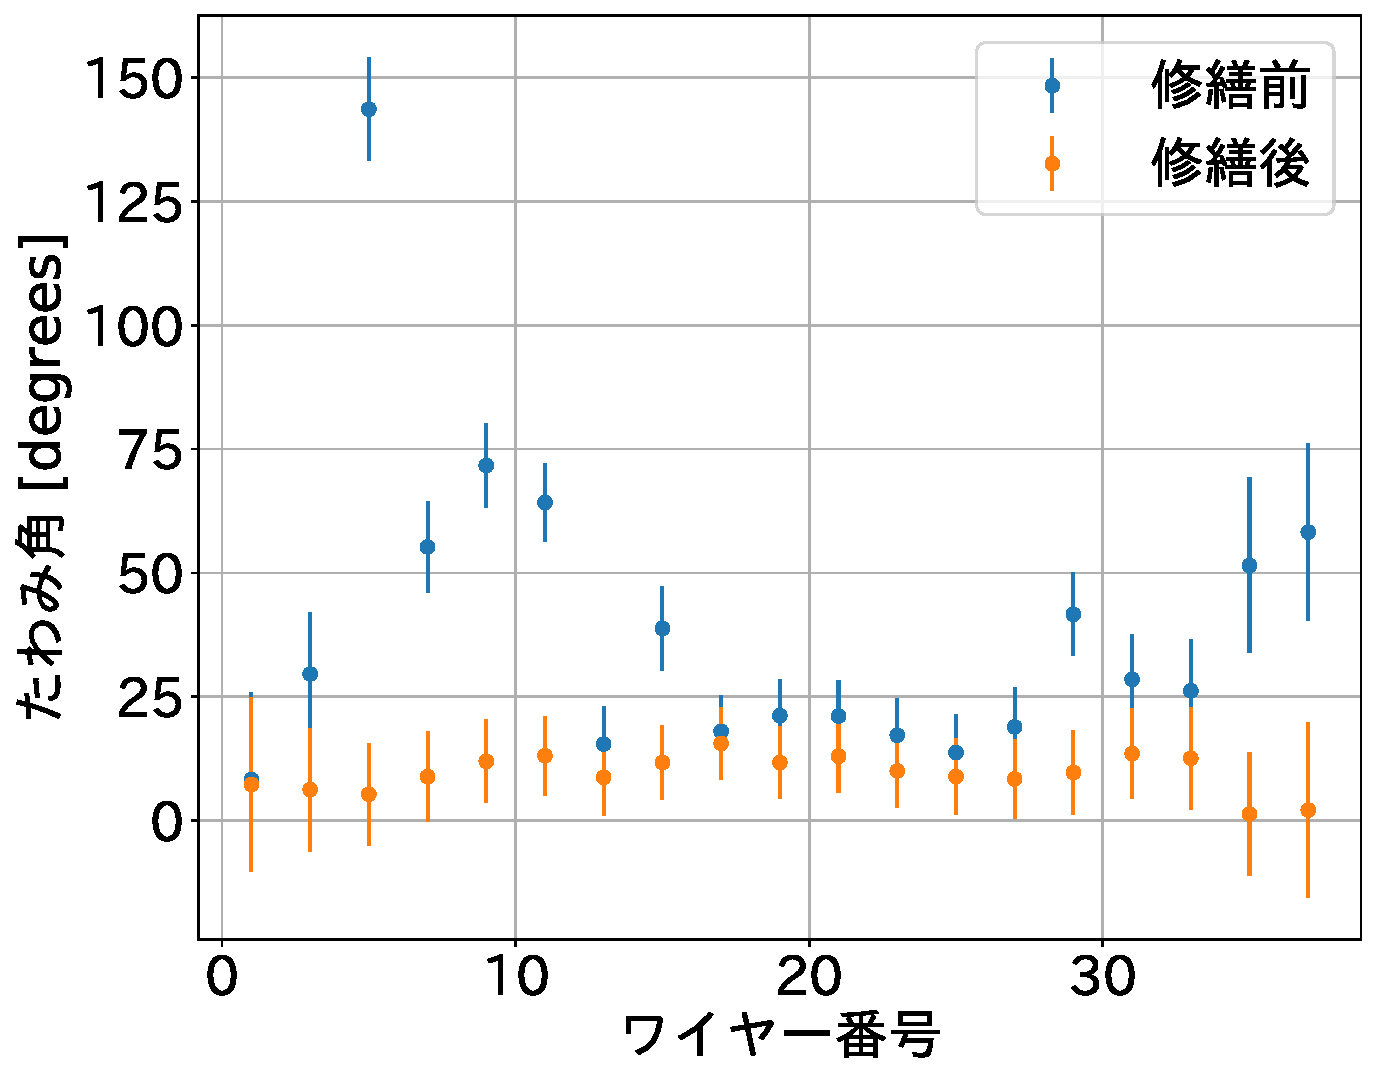
\includegraphics[width=1.0\textwidth]{wiresag_swg/swg_sag_odd_comparison.pdf}
        \subcaption{}
        \label{fig:wiresag_swg_sag_odd_comparison}
    \end{minipage}
    \begin{minipage}[b]{0.5\hsize}
        \centering
        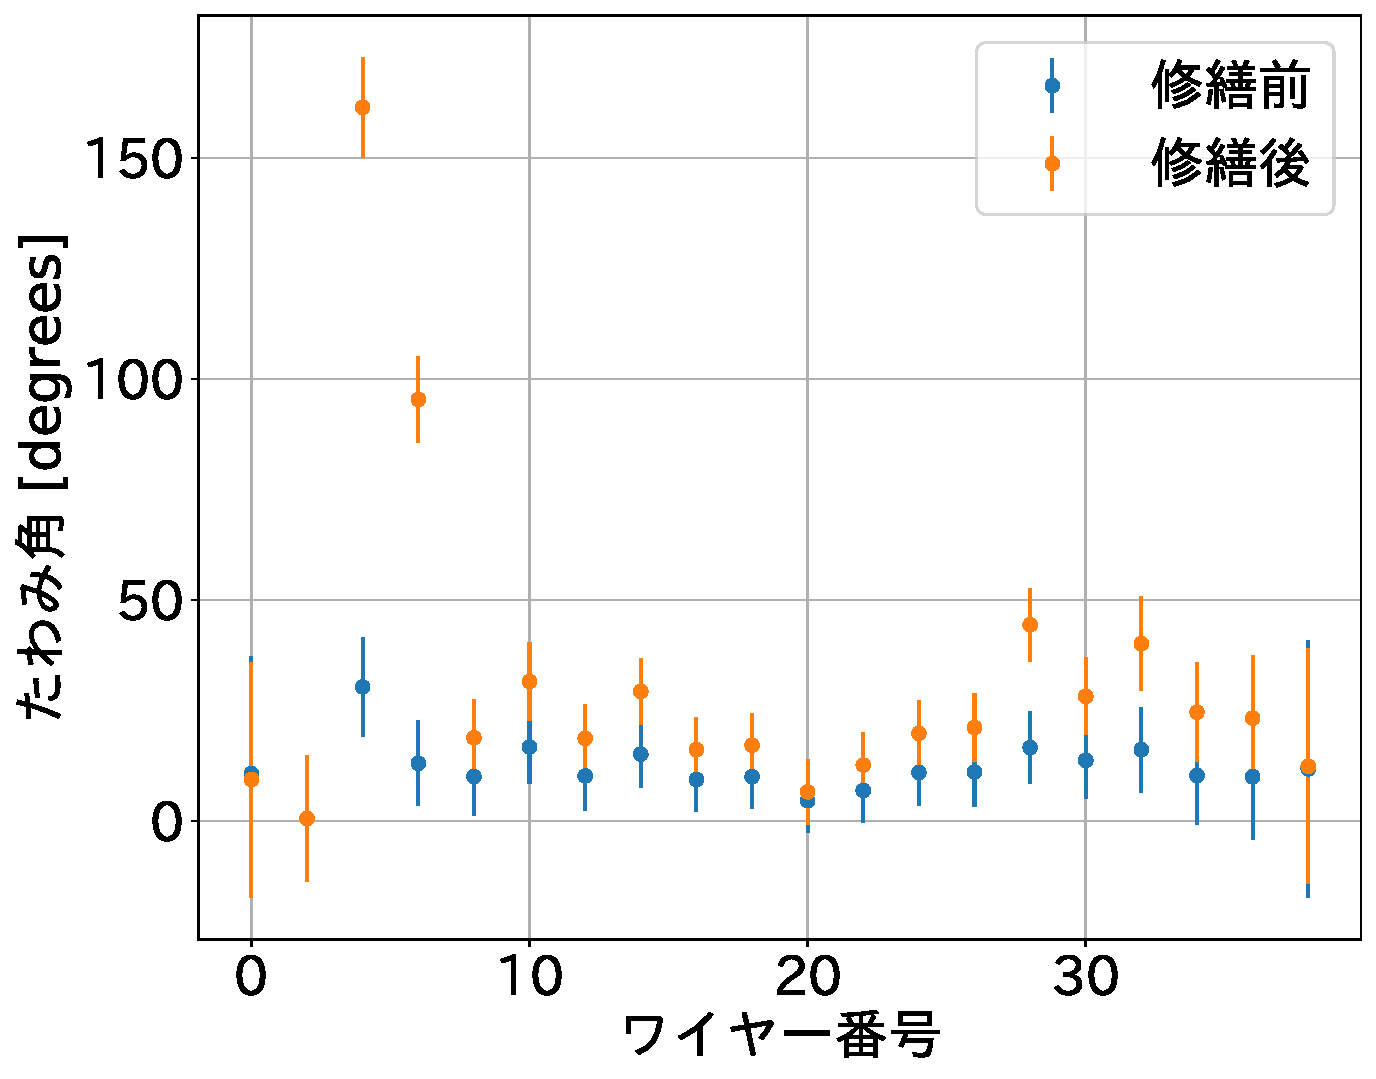
\includegraphics[width=1.0\textwidth]{wiresag_swg/swg_sag_even_comparison.pdf}
        \subcaption{}
        \label{fig:wiresag_swg_sag_even_comparison}
    \end{minipage}
    \caption{(\subref{fig:wiresag_swg_sag_odd_comparison}) 奇数番目のワイヤーのたわみ量の修繕前後での比較。修繕後の方が小さくなっており、改善している。\ 
             (\subref{fig:wiresag_swg_sag_even_comparison}) 偶数番目のワイヤーのたわみ量の修繕前後での比較。
             修繕後の方が大きくなっており、修繕時に張り直されなかったワイヤーはたわみ量が大きくなることを示唆する。
             }
    \label{fig:wiresag_swg_even_odd_repair_comparison}
\end{figure}

\section{まとめと今後の展望}
本章では、開発したワイヤーのたわみ量の自動評価装置を用いて、望遠鏡の偏光角較正に使用されるスパースワイヤーグリッドのたわみ量を評価した。
最初に評価されたワイヤーのたわみ角の平均値は$0.025\tcdegree$であったが、たわみ角が大きいワイヤーを張り直すことでそのたわみ角は$0.020\tcdegree$に改善された。
また、この修繕ではたわみ角が$0.05\tcdegree$を超えるワイヤーが6本存在していたが、修繕後には2本に減少した。
以上から、本装置を用いてたわみ角が大きいワイヤーを選別し、ワイヤーを張り直すことでたわみ角を改善可能であることが示された。
この評価値は先行研究にて与えられる$\theta_{\mathrm{sag}}<0.05\tcdegree$よりも小さく、本装置を用いて
ワイヤーのたわみ量を改善することでたわみ角を$\theta_{\mathrm{sag}}=0.030\tcdegree$程度に抑えることができることが示された。
また、スパースワイヤーグリッドのワイヤーを偶数番目、奇数番目の2回に分けて張ることにより、
先に張られたワイヤーがたわんでしまう可能性があることがわかった。

今後の展望として、まず今回評価したスパースワイヤーグリッドに関して、品質の悪い2本のワイヤーをだけを張り直す。

また、今後新たにスパースワイヤーグリッドにワイヤーを張る際には、すべてのワイヤーを同時に張るように張り方を改善することを提案する。
% たわみ量をさらに抑えるためにはスパースワイヤーグリッドのワイヤーを張る工程を改善することが重要である。
% まずはワイヤーをすべて同時に張ることで、ワイヤーのたわみ量を均一に抑えることができるか調べる必要がある。

% これによりワイヤーがスパースワイヤーグリッドのリングを歪めているかどうかを検証できる。
% また、張力によりワイヤーがスパースワイヤーグリッドのリングを歪めているのであれば、リングの構造を歪みに対して強力なものに変更するか、
% ワイヤーにかける張力を弱めることでさらなるたわみ量の改善が見込まれる。
\end{document}